% Created 2026-05-19 Tue 01:30
% Intended LaTeX compiler: pdflatex
\documentclass[11pt]{article}

\usepackage[utf8]{inputenc}
\usepackage[T1]{fontenc}
\usepackage{graphicx}
\usepackage{longtable}
\usepackage{wrapfig}
\usepackage{rotating}
\usepackage[normalem]{ulem}
\usepackage{amsmath}
\usepackage{amssymb}
\usepackage{capt-of}
\usepackage{hyperref}
\author{Serob Tigranyan}
\date{\today}
\title{Priority Queues and Applications}
\hypersetup{
 pdfauthor={Serob Tigranyan},
 pdftitle={Priority Queues and Applications},
 pdfkeywords={},
 pdfsubject={},
 pdfcreator={},
 pdflang={English}}
\begin{document}

\maketitle
\tableofcontents

\newpage
\section{Introduction}
\label{sec:orgdfeb46e}
A \textbf{Priority Queue} is an abstract data type that operates similarly to a regular queue or stack, but where every element has an associated ``priority.'' In a priority queue, an element with high priority is served before an element with low priority.

\begin{center}
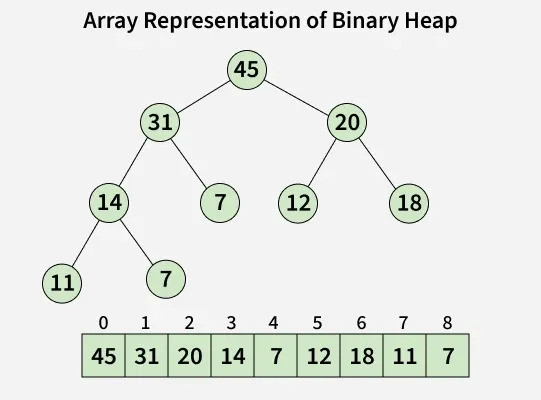
\includegraphics[width=.9\linewidth]{lol.jpg}
\end{center}
\subsection{Implementation: The Binary Heap}
\label{sec:orgc775ace}
In computer science, a priority queue is most efficiently implemented using a \textbf{Binary Heap}.
\subsubsection{What is a Binary Heap?}
\label{sec:orgb907193}
A Binary Heap is a complete binary tree that satisfies the \textbf{heap property}:
\begin{itemize}
\item \textbf{Max-Heap:} The value of each node is less than or equal to the value of its parent. The largest element is at the root.
\item \textbf{Min-Heap:} The value of each node is greater than or equal to the value of its parent. The smallest element is at the root.
\end{itemize}
\subsubsection{Array-Based Implementation}
\label{sec:org0cd3b0f}
Because a heap is a \textbf{complete} binary tree (all levels are filled except possibly the last, which is filled from left to right), it can be stored compactly in a contiguous array without pointers.

For an element at index \texttt{i}:
\begin{itemize}
\item \textbf{Left Child:} \texttt{2i + 1}
\item \textbf{Right Child:} \texttt{2i + 2}
\item \textbf{Parent:} \texttt{(i - 1) / 2}
\end{itemize}

This layout allows for \(O(1)\) access to the top element and \(O(\log n)\) time for both insertion and deletion by ``bubbling'' or ``sifting'' elements up or down to restore the heap property.

\newpage
\section{C++ Support for Priority Queues}
\label{sec:orgd65e60d}
C++ provides built-in support for priority queues through the Standard Template Library (STL).
\subsection{The \texttt{std::priority\_queue} Container}
\label{sec:orgd699af8}
Found in the \texttt{<queue>} header, \texttt{std::priority\_queue} is a container adaptor. It provides \(O(\log n)\) insertion and extraction, and \(O(1)\) access to the top element.

Basic usage of \texttt{std::priority\_queue}:
\begin{verbatim}
#include <iostream>
#include <queue>

int main() {
    // Default: Max heap
    std::priority_queue<int> max_queue;
    // Min heap
    std::priority_queue<
        int, 
        std::vector<int>, 
        std::greater<int>> min_queue;

    for (const int e : { 45, 31, 20, 14, 7, 12, 18, 11, 7, }) {
        max_queue.push(e);
        min_queue.push(e);
    }

    std::cout << "max: ";
    while (!max_queue.empty()) {
        std::cout << max_queue.top() << " ";
        max_queue.pop();
    }
    std::cout << std::endl;
    
    std::cout << "min: ";
    while (!min_queue.empty()) {
        std::cout << min_queue.top() << " ";
        min_queue.pop();
    }
    std::cout << std::endl;

    return 0;
}
\end{verbatim}

Which yields the following output:
\begin{verbatim}
endrohu@noedarlin:/tmp $ c++ -std=c++20 prio_queue.cpp -o queue && ./queue 
max: 45 31 20 18 14 12 11 7 7 
min: 7 7 11 12 14 18 20 31 45
\end{verbatim}
\subsection{Key Properties}
\label{sec:orgd68e689}
\begin{itemize}
\item \textbf{Underlying Container:} Defaults to \texttt{std::vector}, but can use \texttt{std::deque}.
\item \textbf{Ordering:} By default, it uses \texttt{std::less<T>}, making it a \textbf{Max-Heap}.
\item \textbf{No Iterator Support:} Unlike \texttt{std::vector} or \texttt{std::list}, you cannot iterate through a priority queue. You can only access the \texttt{top()} element.

\newpage
\end{itemize}
\section{Technical Challenges: The ``Decrease Key'' Problem}
\label{sec:org380209f}
Standard \texttt{std::priority\_queue} does \textbf{not} support updating the priority of an element already in the queue.
\subsection{Solutions:}
\label{sec:org0703b7a}
\begin{enumerate}
\item \textbf{Lazy Removal:} Instead of updating, push a new entry with the better cost. When popping, check if the node has already been processed with a lower cost; if so, skip it.
\item \textbf{std::make\textsubscript{heap}:} Use a raw \texttt{std::vector} with \texttt{std::push\_heap} and \texttt{std::pop\_heap}, which allows manual searching or using a custom indexed heap.
\end{enumerate}

\newpage
\section{Example Code: Custom Priority Handling}
\label{sec:org09557e4}
\begin{verbatim}
#include <iostream>
#include <queue>
#include <vector>

struct RenderBatch {
    int id;
    int z_index;

    // Min-Heap based on z_index
    bool operator>(const RenderBatch& other) const {
        return z_index > other.z_index;
    }
};

int main() {
    std::priority_queue<RenderBatch,
                        std::vector<RenderBatch>,
                        std::greater<RenderBatch>> draw_queue;

    draw_queue.push({1, 100}); // UI
    draw_queue.push({2, 0});   // Background
    draw_queue.push({3, 50});  // Player

    while (!draw_queue.empty()) {
        RenderBatch batch = draw_queue.top();
        std::cout << "Rendering Batch ID: " << batch.id
                  << " (Z-Index: " << batch.z_index
                  << ")" << std::endl;
        draw_queue.pop();
    }

    return 0;
}
\end{verbatim}
\section{Applications}
\label{sec:org7c0f805}
As a game engine developer, I personally have used priorities queues in the past so I will demonstrate few of its applications in engine development.
Priority queues are vital in game development for managing asynchronous tasks and ensuring deterministic ordering.
\subsection{1. Abstracted Render Command Queues}
\label{sec:org9d42f80}
Modern APIs like Vulkan and DirectX 12 have native \textbf{CommandQueues}. OpenGL, however, is notoriously single-threaded: its context can only be active on one thread at a time.
\begin{itemize}
\item \textbf{The Problem:} How do we allow other threads (AI, Physics, Editor) to ``call'' OpenGL functions?
\item \textbf{The Solution:} We imitate a Command Queue.
\begin{itemize}
\item \textbf{Abstraction:} Create a \texttt{GLCommandQueue} class.
\item \textbf{Submission:} Worker threads call \texttt{gl\_submit\_command} to push commands (e.g., \texttt{DrawMeshCommand}, \texttt{UpdateUniformCommand}) to a thread-safe queue.
\item \textbf{Execution:} The main thread (Render Thread) calls \texttt{gl\_execute\_commands} in a tight loop, popping and executing the actual GL calls.
\end{itemize}
\item \textbf{Role of Priority Queues:} While often a FIFO queue is used for strict ordering, a \textbf{Priority Queue} can be used to prioritize ``Immediate'' commands (like UI or Debug lines) over ``Background'' commands (like texture mipmap generation).

\newpage
\end{itemize}
\subsection{2. Multi-threaded Engine Events}
\label{sec:orgfb77537}
In a complex engine or editor, subsystems (Virtual File System, Input, Windowing) need to communicate across threads.
\begin{itemize}
\item \textbf{Mechanism:} A global \texttt{EventManager} where systems register/subscribe to events (e.g., \texttt{FileChangedEvent}, \texttt{WindowResizeEvent}).
\item \textbf{The Ordering Challenge:} In a multi-threaded environment, events might be submitted nearly simultaneously from different threads. To maintain determinism, events must be processed in the exact order they occurred.
\item \textbf{Priority Queue Usage:} By using a \textbf{Min-Heap} keyed by a high-resolution \textbf{Timestamp}, the engine ensures that a \texttt{WindowResizeEvent} that happened at \(T=10ms\) is always processed before a \texttt{FileChangedEvent} at \(T=11ms\), regardless of which thread pushed them to the queue first.

\newpage
\end{itemize}
\subsection{3. 2D Batch Rendering (Z-Index Sorting)}
\label{sec:orgd227b7b}
In a 2D engine's batch renderer, draw calls must be ordered correctly to handle layering (parallax, UI, sprites).
\begin{itemize}
\item \textbf{Mechanism:} Each batch of sprites or geometry is assigned a \texttt{z\_index}.
\item \textbf{The Problem:} Different systems (UI, Game World, Particle System) submit draw commands in any order, but they must be rendered from back to front.
\item \textbf{Priority Queue Usage:} A \textbf{Min-Heap} stores batches keyed by their \texttt{z\_index}.
\item \textbf{Benefit:} The renderer pops batches in the correct order, ensuring that a ``UI'' batch with a high Z-Index is always drawn on top of a ``Background'' batch with a low Z-Index, regardless of submission order.
\end{itemize}

\newpage
\section{Sources}
\label{sec:orgdcf2ab2}
\begin{itemize}
\item \url{https://www.geeksforgeeks.org/dsa/priority-queue-set-1-introduction/}
\item \url{https://en.cppreference.com/cpp/container/priority\_queue}
\item \url{https://en.wikipedia.org/wiki/Priority\_queue}
\end{itemize}
\end{document}
